\chapter{Feature Extraction}\label{ch:feature_extraction}

\section{Smoothing}{
     Preceding the extraction process a smoothing\footnote{\cref{ch:smoothing}} of the images was performed to enhance the feature quality. For this dataset this was especially important because there was noise as can be seen on the intensity image projection (\cref{fig:intensity}) for example.
}


\section{Comparison Criteria}{
    On top of just extracting the features in this part I also compared different extraction methods and the aforementioned different complementary data types. The criteria for determining the quality of the feature extraction process are the amount of points detected as well as the duplicate rate of features detected repeatedly.
}

\section{Comparison of Extraction Methods}{
    For the extraction and matching procedure I used three different techniques which I wanted to compare regarding extraction, matching and of course in the end the quality of motion estimation.

    \subsection{ORB}{
        The first method considered was ORB \footnote{ORB: An efficient alternative to SIFT or SURF \citep{ORB}} (Oriented FAST and Rotated BRIEF) and as the name suggests it consists of a FAST extractor and then uses the BRIEF method with an additional rotation invariance for the description process.
        In addition to scale and rotational invariance it also provides consistency regarding significant viewpoint change.
    }

    \subsection{BRISK}{
        As a second extraction – matching based method I chose BRISK\footnote{BRISK: Binary Robust Invariant Scalable Keypoints \citep{BRISK}}. Like ORB it is based on the FAST extractor. Similar to BRIEF its descriptor consists of 128 pixel intensity comparisons which for the case of BRISK however is radially symmetric. BRISK shows slower performance than BRIEF, has however the advantage of rotational and scale invariance.
    }

    \subsection{KLT Optical Flow}{
        The last method in my comparison framework was no matching technique but instead the point tracking procedure of optical flow through KLT\footnote{Lucas Kanade Tracking \citep{KLT}}. 
    }
    \clearpage

    \subsection{Visual Comparison}{

        We start of with a visual comparison of the feature extraction on intensity data:

        \begin{figure}[ht]
            \centering
            \subfloat[ORB keypoints]{
                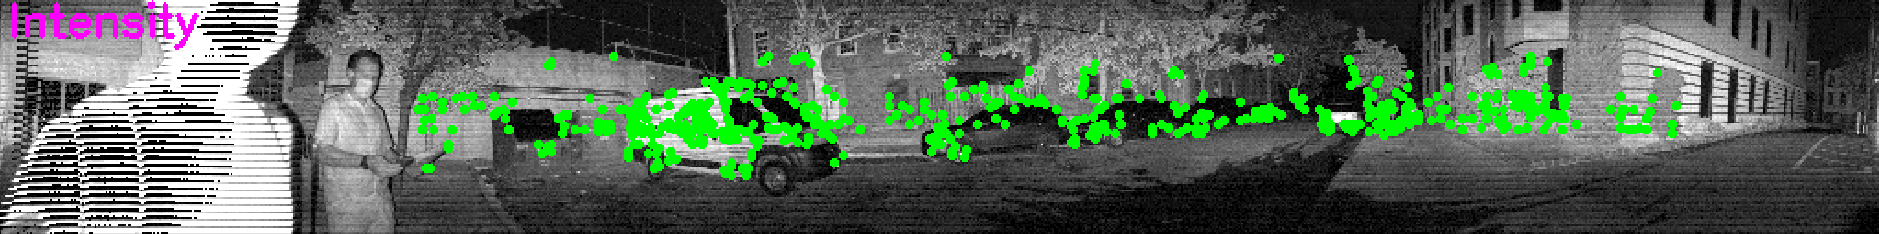
\includegraphics[scale=0.19]{images/extraction/orb.png}
                \label{fig:orb_keypoints}
            }\\
            \subfloat[BRISK keypoints]{
                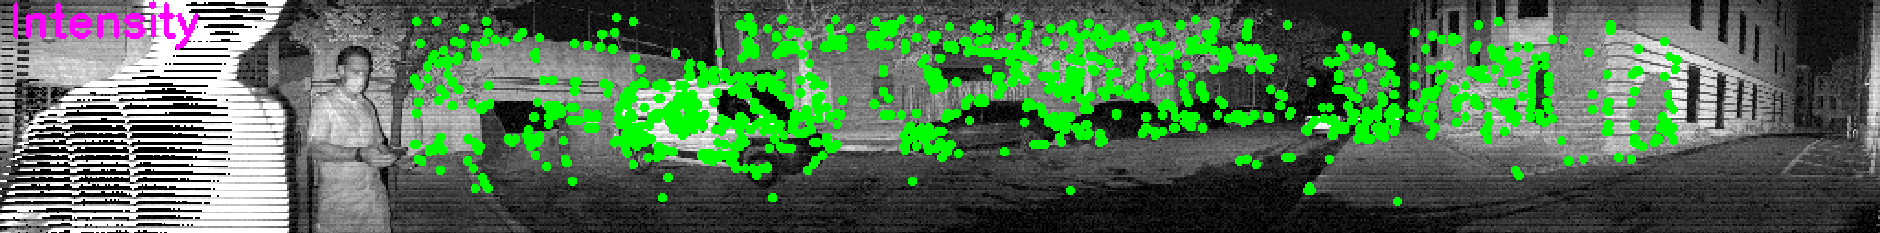
\includegraphics[scale=0.19]{images/extraction/brisk.png}
                \label{fig:brisk_keypoints}
            }\\
            \subfloat[KLT keypoints]{
                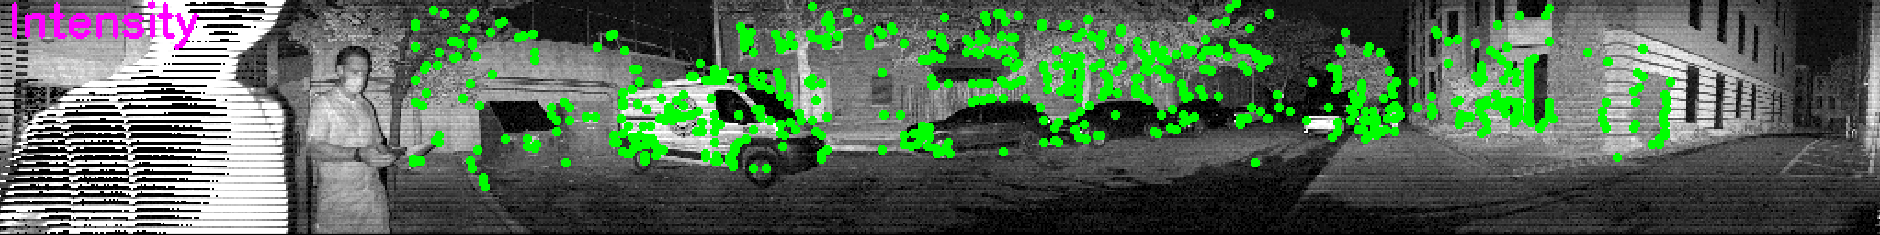
\includegraphics[scale=0.19]{images/extraction/klt.png}
                \label{fig:klt_keypoints}
            }
            \caption{Extractor Comparison}
        \end{figure}

        
        As can be seen on the images, a mask was applied to neglect features detected on the sensor holder or companion.
        From the visual comparison we can see all the methods performing reasonably well regarding the amount of features extracted. What is not visible is the rate of duplicates which was determined by applying a simple duplicate filtering and comparing the numbers.

    }

    \subsection{Statistical Comparison}{

        When considering the extraction results on intensity data over the whole duration of the 20 minute scan (12'000 scans at 10Hz) this is the comparison drawn:

        \begin{table}[!ht]
            \setlength{\extrarowheight}{5pt}
            \centering
            \large
            \begin{tabular}{cccc}
                 & \# Extracted & \# Non-Duplicates & Non-Duplicate Rate\\[12pt]
                \hline
                ORB & 529 & 521 & 98.6\\[12pt]
                \hline
                BRISK & 722 & 699 & 96.8\\[12pt]
                \hline
                KLT & 477 & 477 & 100\\[12pt]
                \hline
            \end{tabular}
            \caption{Extraction Comparison regarding Methods}
            \label{tab:extraction_methods}
        \end{table}
        
        The first result that sticks out is the 100\% non-duplicate rate for KLT which is owed to the fact that KLT has a built-in duplicate rejection mechanism. Apart from that it is worth mentioning that KLT can't be compared exactly to the other methods as it doesn't extract features each step but rather tracks them. With that in mind we see that BRISK extracts significantly more features than ORB and KLT extracts the fewest on average. Lastly overall the duplicate rates seem acceptable. Thus no preference can be voiced so far regarding the different feature methods used.
        
    }


}
\clearpage

\section{Complementary Data Comparison}{
    In the following the ORB method is used on all image types:
    \subsection{Visual Comparison - projection data types}{
    \begin{figure}[ht]
        \centering
        \subfloat[Intensity keypoints]{
            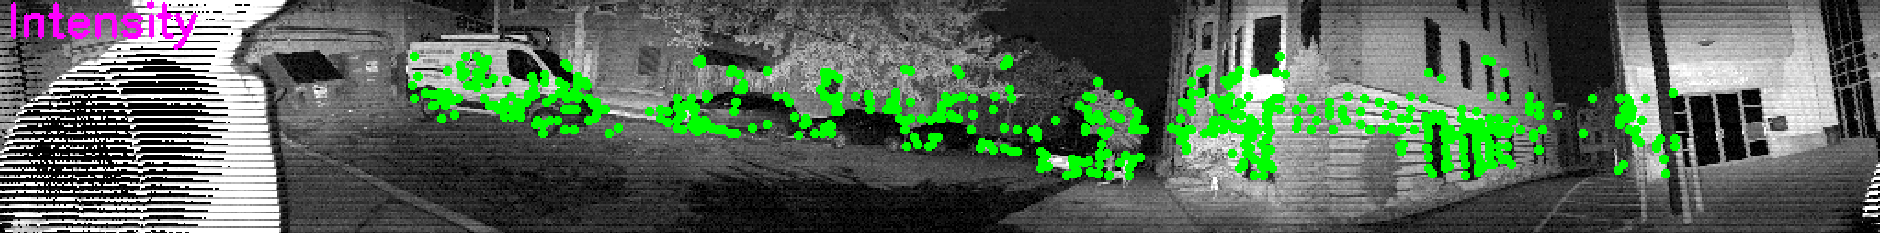
\includegraphics[scale=0.19]{images/extraction/intensity.png}
            \label{fig:intensity_keypoints}
        }\\
        \subfloat[Ambient keypoints]{
            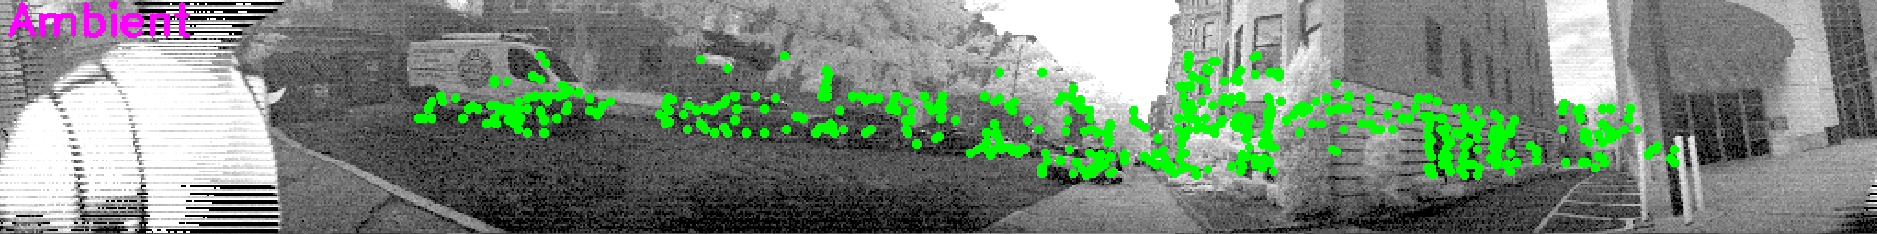
\includegraphics[scale=0.19]{images/extraction/ambient.png}
            \label{fig:ambient_keypoints}
        }\\
        \subfloat[Range keypoints]{
            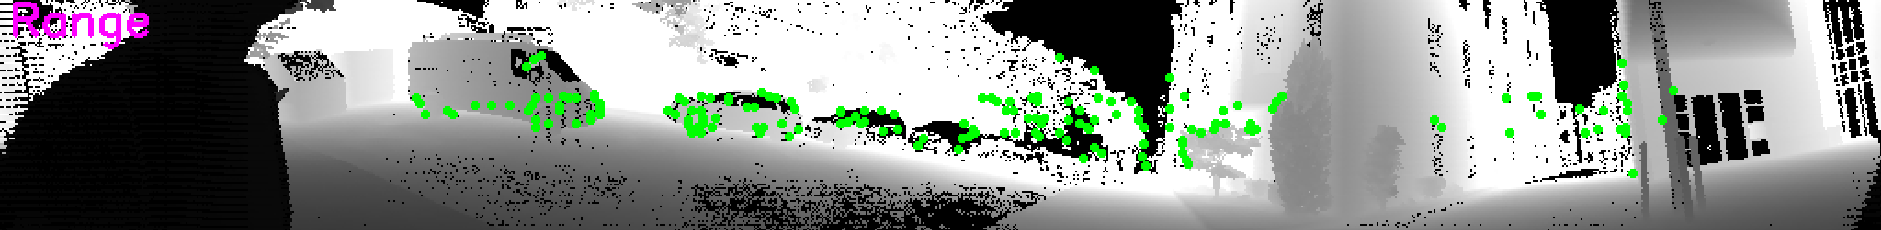
\includegraphics[scale=0.19]{images/extraction/range.png}
            \label{fig:range_keypoints}
        }
        \caption{Extraction Comparison of Complementary Data}
    \end{figure}

    Intensity and ambient both seem to perform well while range detects noticeably fewer points than the other two. Another observation is that the furthest range features result from the gradient of detected to non-reflected points in the sky. These are somewhat artificial features which might already be an indication of suboptimal performance.
    }
    \subsection{Statistical Comparison - projection data types}{

    Considering the average numbers over the whole duration:

    \begin{table}[!ht]
        \setlength{\extrarowheight}{10pt}
        \centering
        \large
        \begin{tabular}{cccc}
             & \# Extracted & \# Non-Duplicates & Non-Duplicate Rate\\[12pt]
            \hline
            Intensity & 529 & 521 & 98.6\\[12pt]
            \hline
            Ambient & 433 & 428 & 98.7\\[12pt]
            \hline
            Range & 256 & 254 & 99.25\\[12pt]
            \hline
        \end{tabular}
        \caption{Extraction Comparison regarding Methods}
        \label{tab:extraction_data}
    \end{table}

    Here the statistics repeat the story of the visual comparison. Intensity and Ambient provide similar numbers of extracted features while on the range image significantly fewer points are detected. However all data types seem viable regarding duplicate detection.

    }

}